%% Wzóra sprawozdania w LateXu

\documentclass[polish,polish,a4paper]{article}
\usepackage[table]{xcolor} % for cell colors
\usepackage{float}
\usepackage[T1]{fontenc}
\usepackage[utf8]{inputenc}
\usepackage{cite}
\usepackage{babel}
\usepackage{amsmath}
\usepackage{graphicx}
\usepackage{pslatex}
\usepackage{wrapfig}
\usepackage{pgfplots}
\usepackage[europeanresistors]{circuitikz} 
\usepackage{subcaption}
\usepackage{anysize}
\usepackage{booktabs, multirow} % for borders and merged ranges
\usepackage{soul}% for underlines

\usepackage{changepage,threeparttable} % for wide tables
\marginsize{2.5cm}{2.5cm}{3cm}{3cm}
\bibliographystyle{IEEEtran}

\newcommand{\PRzFieldDsc}[1]{\sffamily\bfseries\scriptsize #1}
\newcommand{\PRzFieldCnt}[1]{\textit{#1}}
\newcommand{\PRzHeading}[8]{
%% #1 - nazwa laboratorium
%% #2 - kierunek 
%% #3 - specjalność 
%% #4 - rok studiów 
%% #5 - symbol grupy lab.
%% #6 - temat 
%% #7 - numer lab.
%% #8 - skład grupy ćwiczeniowej

\begin{center}
\begin{tabular}{ p{0.32\textwidth} p{0.15\textwidth} p{0.15\textwidth} p{0.12\textwidth} p{0.12\textwidth} }

  &   &   &   &   \\
\hline
\multicolumn{5}{|c|}{}\\[-1ex]
\multicolumn{5}{|c|}{{\LARGE #1}}\\
\multicolumn{5}{|c|}{}\\[-1ex]

\hline
\multicolumn{1}{|l|}{\PRzFieldDsc{Kierunek}}    & \multicolumn{1}{|l|}{\PRzFieldDsc{Specjalność}}   & \multicolumn{1}{|l|}{\PRzFieldDsc{Rok studiów}}   & \multicolumn{2}{|l|}{\PRzFieldDsc{Symbol grupy lab.}} \\
\multicolumn{1}{|c|}{\PRzFieldCnt{#2}}      & \multicolumn{1}{|c|}{\PRzFieldCnt{#3}}        & \multicolumn{1}{|c|}{\PRzFieldCnt{#4}}        & \multicolumn{2}{|c|}{\PRzFieldCnt{#5}} \\

\hline
\multicolumn{4}{|l|}{\PRzFieldDsc{Temat Laboratorium}}      & \multicolumn{1}{|l|}{\PRzFieldDsc{Numer lab.}} \\
\multicolumn{4}{|c|}{\PRzFieldCnt{#6}}              & \multicolumn{1}{|c|}{\PRzFieldCnt{#7}} \\

\hline
\multicolumn{5}{|l|}{\PRzFieldDsc{Skład grupy ćwiczeniowej oraz numery indeksów}}\\
\multicolumn{5}{|c|}{\PRzFieldCnt{#8}}\\

\hline
\multicolumn{3}{|l|}{\PRzFieldDsc{Uwagi}}   & \multicolumn{2}{|l|}{\PRzFieldDsc{Ocena}} \\
\multicolumn{3}{|c|}{\PRzFieldCnt{\ }}      & \multicolumn{2}{|c|}{\PRzFieldCnt{\ }} \\

\hline
\end{tabular}
\end{center}
}

\begin{document}

\PRzHeading{Laboratorium Elektroniki}{Informatyka}{--}{I}{L6}{Tranzystor MOS}{6}{Maciej Kaszkowiak (151856), Dawid Jędraszczyk(148293), Michał Kalinowski(151758)}{}

\section{Cel}

Celem zajęć było zapoznanie się z tranzystorami polowymi pMOS oraz nMOS. Naszym zadaniem od strony teoretycznej było zrozumienie działania podanych tranzystorów, ich zastowosowania i różnic między nimi. Natomiast od strony praktycznej zajęliśmy się tworzeniem podstawowych układów elektoronicznych składających się z między innymi: tranzystora, rezystancji oraz diody, wyznaczaniem napięć w układzie, pobudzaniem układów róznymi sygnałami i częstotliwościami.


\section{nMOS}

\subsection{Charakterystyka bramkowa nMOS}

Zbudowaliśmy następujący układ na płytce prototypowej:
\begin{figure}[H]
\centering
\includegraphics[width=0.55\textwidth]{nmos bramkowa.pdf}
\caption{Układ służący do zmierzenia charakterystyki bramkowej.}
\end{figure}



Uzyskaliśmy następujące pomiary:



\begin{table}[H]
\centering
\caption{Pomiary prądu drenu w zależności od napięcia Bramka - Źródło}\label{tab: }
\begin{tabular}{lrr}\toprule
Napięcie Bramka - Źródło [V] &Prąd drenu [mA] \\\midrule
0.00 &22.00 \\
0.65 &21.22 \\
1.10 &20.38 \\
1.61 &19.33 \\
2.15 &20.73 \\
2.18 &21.77 \\
2.23 &24.46 \\
2.29 &30.22 \\
2.38 &48.00 \\
2.54 &111.00 \\
2.61 &152.00 \\
3.10 &160.16 \\
5.11 &160.50 \\
\bottomrule
\end{tabular}
\end{table}

Napięcie progowe $U_{th}$ tranzystora BS170 zgodnie z notą katalogową należy do przedziału od $0.8$ do $3 V$. \cite{BS170} Typowe napięcie progowe wynosi $2.1 V$, natomiast drogą pomiarów ustaliliśmy napięcie progowe w okolicach wartości $2.2 V$.

\begin{figure}[H]
\centering
\begin{tikzpicture}[scale=1]
\begin{axis}[
title={},
title style={text width=25em},
xlabel={Napięcie Bramka - Źródło [V]},
ylabel={Prąd drenu [mA]},
xmin=0,xmax=5,
ymin=0,ymax=180,
xtick={0,0.5,1,1.5,2,2.5,3,3.5,4,4.5,5},
ytick={0,20,40,60,80,100,120,140,160,180},
legend pos=south east,
ymajorgrids=true,grid style=dashed
]

\addplot[color=red,mark=squares]
coordinates {
(0.00, 22.00)
(0.65, 21.22)
(1.10, 20.38)
(1.61, 19.33)
(2.15, 20.73)
(2.18, 21.77)
(2.23, 24.46)
(2.29, 30.22)
(2.38, 48.00)
(2.54, 111.00)
(2.61, 152.00)
(3.10, 160.16)
(5.11, 160.50)
};


\addplot[thick, samples=50, smooth,domain=0:6,magenta] coordinates {(2.1,0)(2.1,180)};

\legend{Id [mA]}
\end{axis}
\end{tikzpicture}
\caption{Napięcie progowe tranzystora nMOS z naniesionym typowym napięciem progowym.}
\end{figure}

Wniosek: aby tranzystor nMOS zaczął przewodzić prąd, napięcie bramki względem masy musi osiągnąć wartość większą od napięcia progowego. \cite{proste} W naszym konkretnym przypadku napięcie musi być w przybliżeniu wyższe niż $2.2V$.


\subsection{Charakterystyka drenowa nMOS}

Zbudowaliśmy następujący układ na płytce prototypowej:

\begin{figure}[H]
\centering
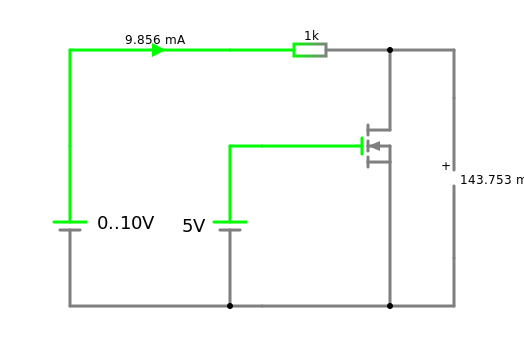
\includegraphics[width=0.55\textwidth]{nmos drenowa.pdf}
\caption{Układ służący do zmierzenia charakterystyki drenowej.}
\end{figure}

Uzyskaliśmy następujące pomiary:

\begin{table}[H]
\centering
\begin{tabular}{|c|c|c|}
\hline
Napięcie na zasilaczu[V] & U\_ds [mV] & I\_d [mA] \\
\hline
1&17.5 & 0.982 \\
\hline
2 &35.4 & 2 \\
\hline
3 &53.1 & 2.95 \\
\hline
4 &71 & 3.94 \\
\hline
5 &89 & 4.92 \\
\hline
6 &107.3 & 5.9 \\
\hline
7 &125.5 & 6.88 \\
\hline
8 &143.9 & 7.86 \\
\hline
9 &163 & 38.84 \\
\hline
10 &182 & 9.91 \\
\hline
\end{tabular}
\caption{Prąd drenu względem napięcia dren - źródło.}
\end{table}

\begin{figure}[H]
\centering
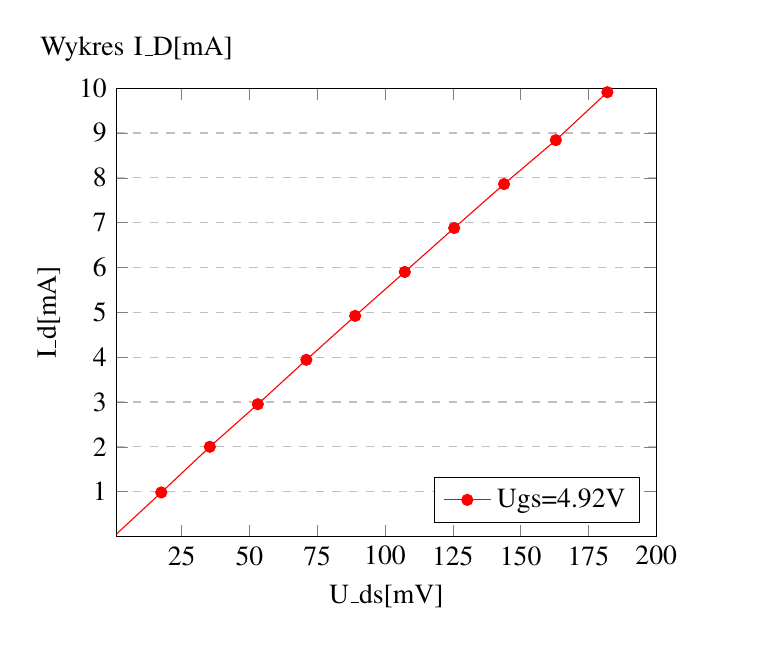
\begin{tikzpicture}
\begin{axis}[
title={Wykres I\_D[mA]},
title style={text width=25em},
xlabel={U\_ds[mV]},
ylabel={I\_d[mA]},
xmin=1,xmax=200,
ymin=0,ymax=10,
xtick={25,50,75,100,125,150,175,200},
ytick={1,2,3,4,5,6,7,8,9,10},
legend pos=south east,
ymajorgrids=true,grid style=dashed
]

\addplot[color=red,mark=*]
coordinates {
(0,0)
(17.5,0.982)
(35.4,2)
(53.1,2.95)
(71,3.94)
(89,4.92)
(107.3,5.9)
(125.5,6.88)
(143.9,7.86)
(163,8.84)
(182,9.91)
};

\legend{Ugs=4.92V}
\end{axis}
\end{tikzpicture}
\caption{Prąd drenu względem napięcia dren - źródło.}
\end{figure}

Zmodyfikowaliśmy powyższy układ w celu wyznaczenia charakterystyki drenowej dla obniżonego napięcia bramki:
\begin{figure}[H]
\centering
\includegraphics[width=0.55\textwidth]{nmos drenowa obnizona.pdf}
\caption{Układ służący do zmierzenia charakterystyki drenowej dla obniżonego napięcia bramki.}
\end{figure}

Uzyskaliśmy następujące pomiary:


\begin{table}[H]
\centering
\begin{tabular}{|c|c|c|}
\hline
Napięcie na zasilaczu[V] & U\_ds [mV] & I\_d [mA]  \\
\hline
1&15.5 & 0.892 \\
\hline
2 &28.4 & 1.84 \\
\hline
3 &41 & 2.77 \\
\hline
4 &63 & 3.76 \\
\hline
5 &76 & 4.72 \\
\hline
6 &89.4 & 5.72 \\
\hline
7 &113.5 & 6.69 \\
\hline
8 &126.8 & 7.66 \\
\hline
9 &149.2 & 8.63 \\
\hline
10 &167.3 & 9.72 \\
\hline
\end{tabular}
\caption{Prąd drenu względem napięcia dren - źródło przy obniżonym napięciu bramki.}
\end{table}

\begin{figure}[H]
\centering
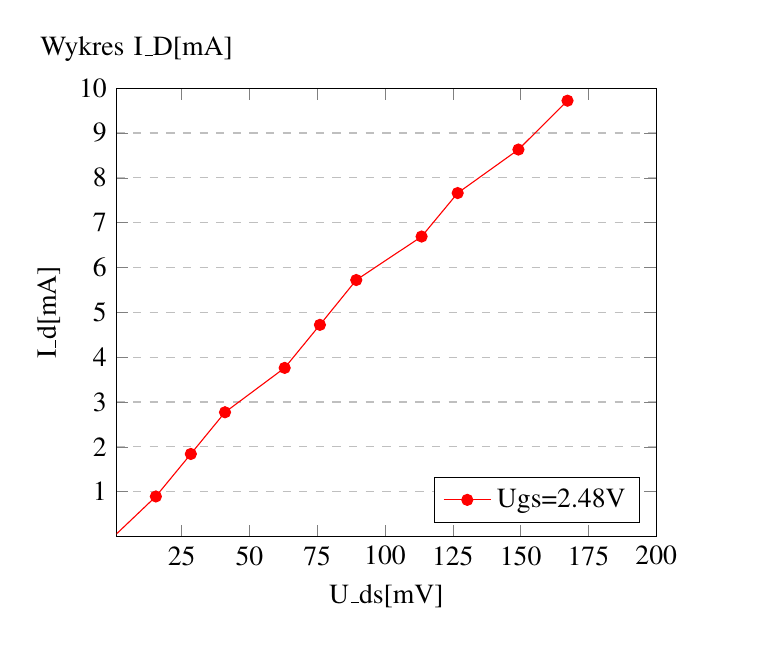
\begin{tikzpicture}
\begin{axis}[
title={Wykres I\_D[mA]},
title style={text width=25em},
xlabel={U\_ds[mV]},
ylabel={I\_d[mA]},
xmin=1,xmax=200,
ymin=0,ymax=10,
xtick={25,50,75,100,125,150,175,200},
ytick={1,2,3,4,5,6,7,8,9,10},
legend pos=south east,
ymajorgrids=true,grid style=dashed
]

\addplot[color=red,mark=*]
coordinates {
(0,0)
(15.5,0.892)
(28.4,1.84)
(41,2.77)
(63,3.76)
(76,4.72)
(89.4,5.72)
(113.5,6.69)
(126.8,7.66)
(149.2,8.63)
(167.3,9.72)
};

\legend{Ugs=2.48V}
\end{axis}
\end{tikzpicture}
\caption{Prąd drenu względem napięcia dren - źródło przy obniżonym napięciu bramki.}
\end{figure}

Możemy przedstawić powyższe wyniki na wspólnym wykresie:
\begin{figure}[H]
\centering
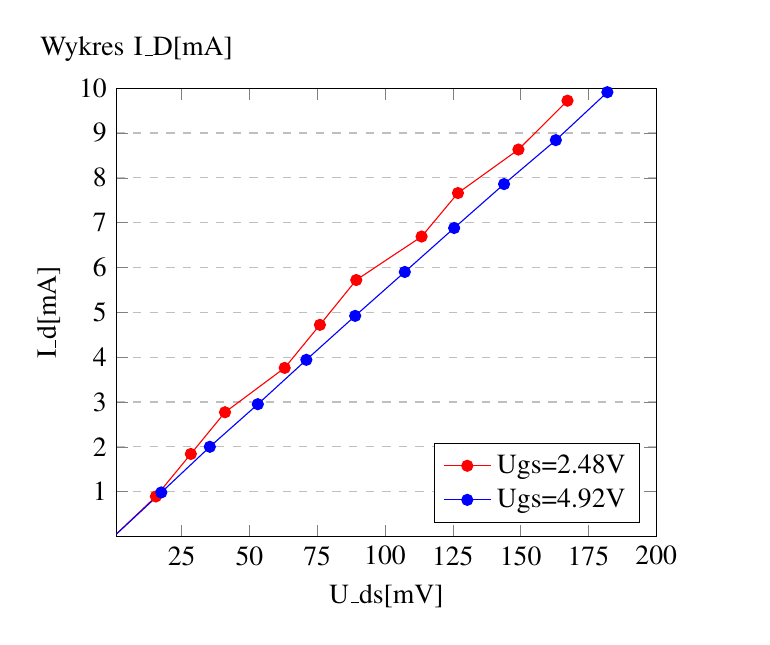
\begin{tikzpicture}
\begin{axis}[
title={Wykres I\_D[mA]},
title style={text width=25em},
xlabel={U\_ds[mV]},
ylabel={I\_d[mA]},
xmin=1,xmax=200,
ymin=0,ymax=10,
xtick={25,50,75,100,125,150,175,200},
ytick={1,2,3,4,5,6,7,8,9,10},
legend pos=south east,
ymajorgrids=true,grid style=dashed
]

\addplot[color=red,mark=*]
coordinates {
(0,0)
(15.5,0.892)
(28.4,1.84)
(41,2.77)
(63,3.76)
(76,4.72)
(89.4,5.72)
(113.5,6.69)
(126.9,7.66)
(149.2,8.63)
(167.3,9.72)
};
\addplot[color=blue,mark=*]
coordinates {
(0,0)
(17.5,0.982)
(35.4,2)
(53.1,2.95)
(71,3.94)
(89,4.92)
(107.3,5.9)
(125.5,6.88)
(143.9,7.86)
(163,8.84)
(182,9.91)
};

\legend{Ugs=2.48V,Ugs=4.92V}
\end{axis}
\end{tikzpicture}
\caption{Prąd drenu względem napięcia dren - źródło w zależności od napięcia bramki.}
\end{figure}

Wniosek:
Wraz ze wzrostem napięcia na bramce zwiększa się prąd drenu I\_d i napięcie źródła U\_ds. Obie te wartości rosną liniowo.

Napięcie progowe $U_{th}$ tranzystora BS170 zgodnie z notą katalogową należy do przedziału od $0.8$ do $3 V$. Typowe napięcie progowe wynosi $2.1 V$, natomiast drogą pomiarów ustaliliśmy napięcie progowe w okolicach wartości $2.2 V$.

\subsection{Tranzystor nMOS jako przełącznik}

Zbudowaliśmy następujący układ na płytce prototypowej:
\begin{figure}[H]
\centering
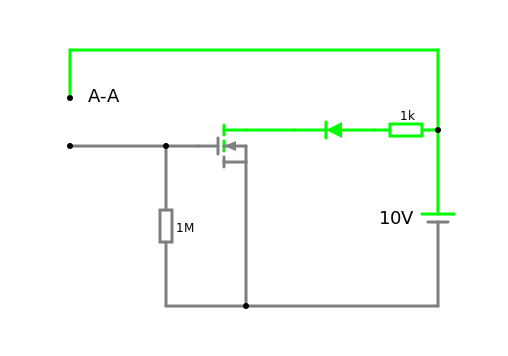
\includegraphics[width=0.55\textwidth]{nmos przelacznik.pdf}
\caption{Układ służący do badania tranzystora nMOS w roli przełącznika}
\end{figure}

Następnie zmodyfikowaliśmy powyższy układ w celu wprowadzenia opóźnienia wyłączania:
\begin{figure}[H]
\centering
\includegraphics[width=0.55\textwidth]{nmos przelacznik opoznienie.pdf}
\caption{Układ służący do pokazania opóźnienia wyłączenia.}
\end{figure}

Dany układ działa jak wyłącznik czasowy, czyli kiedy dokonamy chwilowego zwarcia wyprowadzeń A-A i przestaniemy to układ będzie działał jeszcze chwile, aż do wyczerpania kondensatora. Po jego wyczerpaniu bramka się zamknie tworząc dziure w obwodzie. W praktyce można go na przykład wykorzystać w klatkach schodowych w lampie, która po wejściu mieszkańca pali się jeszcze przez określony czas albo w zamku drzwi, który otwiera się na określony czas po wpisaniu kodu.

\subsection{Czas załączania tranzystora nMOS}

Zbudowaliśmy następujący układ na płytce prototypowej:
\begin{figure}[H]
\centering
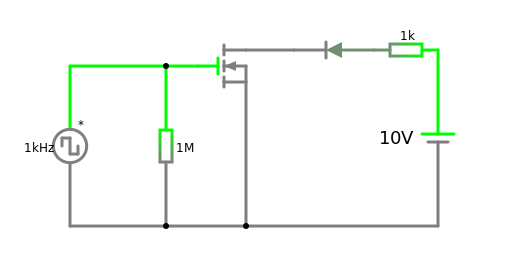
\includegraphics[width=0.55\textwidth]{nmos czas zalaczania.pdf}
\caption{Układ służący do zbadania jasności diody LED w zależności od wypełnienia sygnału PWM.}
\end{figure}

Ustawiliśmy częstotliwość pobudzenia $3 kHz$. Zmieniając wypełnienie sygnału PWM mogliśmy zaobserwować, że większe wypełnienie sygnału sterującego przekładało się na większą jasność świecenia diody LED.

\begin{figure}[H]
\centering
\includegraphics[width=1.0\textwidth]{oscylogram male wypelnienie.png}
\caption{Oscylogram dla małego stopnia wypełnienia sygnału.}
\end{figure}

\begin{figure}[H]
\centering
\includegraphics[width=1.0\textwidth]{oscylogram duze wypelnienie.png}
\caption{Oscylogram dla dużego stopnia wypełnienia sygnału.}
\end{figure}

Następnie ustawiliśmy częstotliwość pobudzenia na poziom $1.25 MHz$. Przy pomocy oscyloskopu ustaliliśmy, że wartość opóźnienia w przełączeniach tranzystora BS170 wynosi $88ns$.

\begin{figure}[H]
\centering
\includegraphics[width=1.0\textwidth]{oscylogram opoznienie.png}
\caption{Oscylogram przedstawiający opóźnienie w przełączeniach tranzystora.}
\end{figure}

\section{pMOS}
\subsection{Charakterystyka bramkowa pMOS}


Zbudowaliśmy następujący układ na płytce prototypowej:
\begin{figure}[H]
\centering
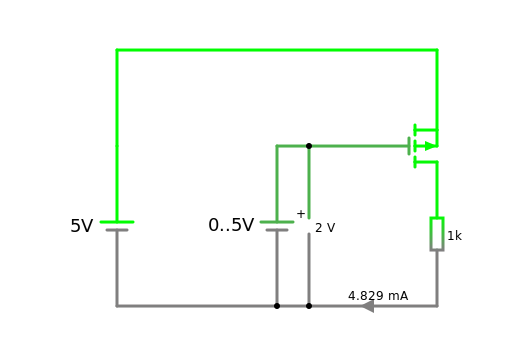
\includegraphics[width=0.55\textwidth]{pmos bramkowa.pdf}
\caption{Układ służący do zmierzenia charakterystyki bramkowej.}
\end{figure}

Uzyskaliśmy następujące pomiary:

\begin{table}[H]\centering
\caption{Prąd drenu w zależności od napięcia na zasilaczu V1.}\label{tab: }
\begin{tabular}{lrr}\toprule
Napięcie na zasilaczu V1 [V] &Prąd drenu [mA] \\\midrule
0.8400 &5.0500 \\
1.4000 &5.0500 \\
2.1000 &5.0500 \\
2.6400 &5.0520 \\
3.1200  &4.0570 \\
3.4000 &3.2000 \\
3.5000 &2.1000 \\
3.9000 &0.1600 \\
4.2000 &0.0000 \\
4.3000 &0.0000 \\
4.6000 &0.0000 \\
5.0000 &0.0000 \\
\bottomrule
\end{tabular}
\end{table}

Zgodnie z prawem Kirchoffa ustaliliśmy, że:
\begin{gather}
U1 = 5V \\
U2 = 0..5V \\
Ugs = U2 - U1 
\end{gather}

Uzyskana zależność przedstawia się następująco:

\begin{figure}[H]
\centering
\begin{tikzpicture}[scale=1]
\begin{axis}[
title={},
title style={text width=25em},
xlabel={Napięcie Bramka - Źródło [V]},
ylabel={Prąd drenu [mA]},
xmin=-5,xmax=0.15,
ymin=0,ymax=0.16,
xtick={-5, -4.5, -4, -3.5, -3, -2.5, -2, -1.5, -1, -0.5, 0},
yticklabel style={
        /pgf/number format/fixed,
        /pgf/number format/precision=5
},
scaled y ticks=false,
legend pos=south east,
ymajorgrids=true,grid style=dashed
]

\addplot[color=red,mark=squares]
coordinates {
(-5, 0.14)
(-3.84, 0.14)
(-3.39, 0.14)
(-3.09, 0.13)
(-2.86, 0.1)
(-2.79, 0.09)
(-2.58, 0.06)
(-2.42, 0.04)
(-1.86, 0.05)
(0.15, 0.04)
};


\addplot[thick, samples=50, smooth,domain=0:6,magenta] coordinates {(-2.1,0)(-2.1,1)};

\legend{Id [mA]}
\end{axis}
\end{tikzpicture}
\caption{Napięcie progowe tranzystora pMOS z naniesionym typowym napięciem progowym.}
\end{figure}


Napięcie progowe $U_{th}$ tranzystora 2N7000 zgodnie z notą katalogową należy do przedziału od $-3 V$ do $-0.8 V$. \cite{2N7000} Typowe napięcie progowe wynosi $-2.1 V$, natomiast drogą pomiarów ustaliliśmy napięcie progowe w okolicach wartości $-2.6 V$.


\subsection{Charakterystyka drenowa pMOS}

Zbudowaliśmy następujący układ na płytce prototypowej:
\begin{figure}[H]
\centering
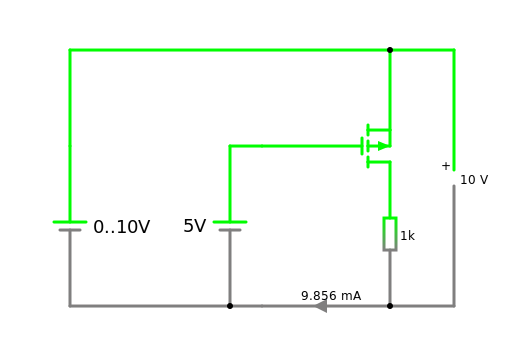
\includegraphics[width=0.55\textwidth]{pmos drenowa.pdf}
\caption{Układ służący do zmierzenia charakterystyki drenowej.}
\end{figure}

Otrzymaliśmy następujące pomiary:

\begin{table}[H]\centering
\caption{Wartość prądu drenu w zależności od napięcia drenu}\label{tab: }
\begin{tabular}{lrr}\toprule
Napięcie Dren - Źródło [V] &Prąd drenu [mA] \\\midrule
-1.1000 &0.5100 \\
-2.2000 &1.4920 \\
-3.1440 &2.4300 \\
-4.2500 &3.5300 \\
-5.1350 &4.4620 \\
-6.2300 &5.6400 \\
-7.2100 &6.8920 \\
-8.0100 &8.2120 \\
-9.9450 &9.1230 \\
-10.0230 &10.2170 \\

\bottomrule
\end{tabular}
\end{table}


Zmodyfikowaliśmy powyższy układ w celu wyznaczenia charakterystyki drenowej dla obniżonego napięcia bramki:
\begin{figure}[H]
\centering
\includegraphics[width=0.55\textwidth]{pmos drenowa obnizona.pdf}
\caption{Układ służący do zmierzenia charakterystyki drenowej dla obniżonego napięcia bramki.}
\end{figure}

\begin{table}[H]\centering
\caption{Wartość prądu drenu w zależności od napięcia drenu}\label{tab: }
\begin{tabular}{lrr}\toprule
Napięcie Dren - Źródło [V] &Prąd drenu [mA] \\\midrule
-1.1230 & 0.0000 \\
-2.2300 & 0.0000 \\
-3.1200 & 0.0000 \\
-4.3200 & 0.0000 \\
-5.2600 & 0.0000 \\
-6.7300 & 0.0000 \\
-7.2100 & 1.7200 \\
-8.1800 & 8.2200 \\
-9.2560 & 9.2930 \\
-10.1980 & 10.2530 \\

\bottomrule
\end{tabular}
\end{table}

\begin{figure}[H]
\centering
\begin{tikzpicture}
\begin{axis}[
title={Zależność wartości prądu drenu od napięcia Dren - Źródło},
xlabel={Napięcie [V]},
ylabel={Prąd drenu [mA]},
xmin=-10.1980, xmax=0,
ymin=0, ymax=10.2530,
xtick={0, -2, -4, -6, -8, -10},
ytick={0,2,4,6,8,10},
legend pos=south east,
ymajorgrids=true,
grid style=dashed,
]

\addplot[
color=blue,
mark=square,
]
coordinates {
(-1.1230, 0.0000)(-2.2300, 0.0000)(-3.1200, 0.0000)(-4.3200, 0.0000)(-5.2600, 0.0000)(-6.7300, 0.0000)(-7.2100, 1.7200)(-8.1800, 8.2200)(-9.2560, 9.2930)(-10.1980, 10.2530)
};
\addlegendentry{$U_{GS}$ = 2.41},

\addplot[
color=red,
mark=square,
]
coordinates {
(-1.1000, 0.5100)(-2.2000, 1.4920)(-3.1440, 2.4300)(-4.2500, 3.5300)(-5.1350, 4.4620)(-6.2300, 5.6400)(-7.2100, 6.8920)(-8.0100, 8.2120)(-10.0230, 10.2170)
};
\addlegendentry{$U_{GS}$ = 4.85},

\end{axis}
\end{tikzpicture} 
\end{figure}

Wniosek: wyższe napięcie bramka - źródło powinno spowodować wzrost napięcia progowego dren - źródło, przy którym wartość prądu powinna gwałtownie się zmienić. Niestety nie zaobserwowaliśmy tego drogą pomiarów ze względu na źle przeprowadzone pomiary. Wniosek wysunęliśmy na podstawie zasymulowania układu. 


\section{Wnioski}

Zaznajomiliśmy się z różnicami w budowie i zastosowaniu między podanymi tranzystorami, np. warunków koniecznych, żeby przez tranzystory płynął prąd.Poznaliśmy definicje prądu drenu, nasycenia oraz odcięcia. Zauważyliśmy różnice w zachowaniach tranzystorów pMOS i nMOS dla różnych napięć, sygnałów i częstotliwości. 

\newpage

\tableofcontents

\bibliography{refs}

\end{document}

